% Nicholas Arnold
% Steven Braeger
% CDA 5106
%
% Project Final Report
%
% We used the template from IEEE website, linked from
% http://www.ieee.org/conferences_events/conferences/publishing/templates.html	

\documentclass[conference]{IEEEtran}
\usepackage{algorithm}
\usepackage{algorithmic}
\usepackage{array}
\usepackage{enumerate}

% *** CITATION PACKAGES ***
%
%\usepackage{cite}
% cite.sty was written by Donald Arseneau
% V1.6 and later of IEEEtran pre-defines the format of the cite.sty package
% \cite{} output to follow that of IEEE. Loading the cite package will
% result in citation numbers being automatically sorted and properly
% "compressed/ranged". e.g., [1], [9], [2], [7], [5], [6] without using
% cite.sty will become [1], [2], [5]--[7], [9] using cite.sty. cite.sty's
% \cite will automatically add leading space, if needed. Use cite.sty's
% noadjust option (cite.sty V3.8 and later) if you want to turn this off.
% cite.sty is already installed on most LaTeX systems. Be sure and use
% version 4.0 (2003-05-27) and later if using hyperref.sty. cite.sty does
% not currently provide for hyperlinked citations.
% The latest version can be obtained at:
% http://www.ctan.org/tex-archive/macros/latex/contrib/cite/
% The documentation is contained in the cite.sty file itself.

% *** MATH PACKAGES ***
%
%\usepackage[cmex10]{amsmath}
% *** SPECIALIZED LIST PACKAGES ***
%
%\usepackage{algorithmic}
% algorithmic.sty was written by Peter Williams and Rogerio Brito.
% This package provides an algorithmic environment fo describing algorithms.
% You can use the algorithmic environment in-text or within a figure


% *** ALIGNMENT PACKAGES ***
%
%\usepackage{array}
%\usepackage{mdwmath}
%\usepackage{mdwtab}
%\usepackage{eqparbox}

% *** SUBFIGURE PACKAGES ***
%\usepackage[tight,footnotesize]{subfigure}

%\usepackage[caption=false]{caption}
%\usepackage[font=footnotesize]{subfig}
%\usepackage{fixltx2e}
%\usepackage{stfloats}
% stfloats.sty was written by Sigitas Tolusis. This package gives LaTeX2e
% the ability to do double column floats at the bottom of the page as well
% as the top. (e.g., "\begin{figure*}[!b]" is not normally possible in
% LaTeX2e). It also provides a command:
%\fnbelowfloat
% to enable the placement of footnotes below bottom floats (the standard
% LaTeX2e kernel puts them above bottom floats). This is an invasive package

% Other Packages
\usepackage{moreverb}
\usepackage{graphicx}
\usepackage{caption}
\usepackage{url}

% correct bad hyphenation here
\hyphenation{op-tical net-works semi-conduc-tor}


\begin{document}
%
% paper title
% can use linebreaks \\ within to get better formatting as desired
\title{SIMT Something Title}


% author names and affiliations
% use a multiple column layout for up to three different
% affiliations
\author{\IEEEauthorblockN{Steven Braeger}
\IEEEauthorblockA{Department of Electrical Engineering and\\Computer Science\\
University of Central Florida\\
Orlando, Florida 32826\\
Email: \texttt{steve@soapforge.com}}
\and\IEEEauthorblockN{Nicholas Arnold}
\IEEEauthorblockA{Department of Electrical Engineering and\\Computer Science\\
University of Central Florida\\
Orlando, Florida 32826\\
Email: \texttt{narnold@knights.ucf.edu}}
}

\maketitle


\begin{abstract} 

\end{abstract}

\IEEEpeerreviewmaketitle


\section{Introduction}



\section{Related Work}

\subsection{Branch Prediction}

We first wanted to take a look at some techniques being researched about how to structure branch predictors in order to see if there were any innovations that would perform better over what we had already learned in class.  We came across a paper by Yeh and Patt \cite{Yeh91}.  They discussed implementing an adaptive branch predictor that would use information being collected at runtime, as opposed to other schemes which would require a pre-run of the program for training.  Their setup requires a Branch History Table and a Branch History Pattern Table, which is updated based on the outcomes of the branches during run-time.  This seemed useful to use due to the fact that their approach would be utilizing run-time information, which is something we are striving to utilize, as well.

Another branch prediction paper we came across was by Eden and Mudge \cite{yags98}.  They developed YAGS, or Yet Another Global Scheme, which is a combination of several strong points of previously implemented schemes.  Using information from implementations such as GShare, the Agree Predictor, the Bi-Mode Predictor, the Skewed Branch Predictor, and the Filter Mechanism, the authors use some schemes to implement a predictor to store the biases of branches and other schemes to implement a predictor to store the direction of those branches.  This seemed useful to us because the two varieties of predictor catch not only the regular behavior of branches, but also the special cases instead of just allowing them to be mispredictions.

In a paper by Pan, So, and Rahmeh \cite{Pan92}, we saw another attempt at improved branch prediction, this time by referencing a subhistory of branch in addition to the branch history table itself.  They claim that by adding only a shift register to the architecture, they were able to achieve an additional 11\% prediction accuracy.  This was interesting to us because it potentially showed us another way we could increase our own accuracy without a vast amount of extra hardware.

\subsection{GPU Architectures}

We next wanted to look at a variety of GPU architecture literature to see what is currently being done on the GPU with regards to branch prediction.  We found several SIGGRAPH course presentations which gave us a large amount of information about GPU architectures \cite{Luebke08, Sig07, Sig09}.  In the NVIDIA Research presentation \cite{Luebke08}, we learned that the GPU architecture has become less and less hardward bound as more and more parts of the GPU pipeline are allowing user programmability.  This presentation also gave us some insight as to how the GPU assigns threads to cores in groups called 'warps'.

The SIGGRAPH 2009 course \cite{Sig09} showed in more detail the hardware differences between CPUs and GPUs.  It also showed us how the GPU handles the large amount of elements assigned to each core and how they currently avoid stalls due to branches.  The fact is, they don't handle stalls at all - when they encounter a branch, they just switch do a different context group and execute the same set of instructions they just completed on the previous group.  Once the GPU has finished doing this chuck of each context group, the branch from the first context group has most of the time been resolved and is ready to continue.

The SIGGRAPH 2007 talk \cite{Sig07} talks more about the progression of the use of GPUs becoming more and more commonplace due to the additional programmability.  It also had a discussion about generalizing the GPU pipeline to allow for better understanding and interactions between varying GPU architectures.  This is important to us because if different GPU architects are not working under some sort of uniformity, then our work here might have vastly different outcomes down the road based on the hardware selection.

\subsection{Branch Prediction on GPU}

We found one paper of someone who previously attempted to do some type of branch prediction on the GPU.  He and Zhang \cite{Zhang09} attempted to use a GPU, which has a many-core architecture, to test out parallel branch prediction for future use in general purpose many-core CPUs.  Their goals were to get independent branch predictors operating on different cores to cooperate with each other in an effort to:

\begin{enumerate}
	\item increase prediction accuracy,
	\item dynamically combine predictors to make them more powerful, or
	\item switch them off if they are behaving the same in order to save power.
\end{enumerate}

This paper caught our attention because it involved branch prediction on the GPU, but we realized that the authors were using the GPU to test CPU-style computations, and our goals are to try and use branch prediction to improve GPU-style computations using GPU workflows.

\section{Technical Sections}

In general, CPU architecture is different than GPU architecture in a few ways.  CPU architecture includes logic for the fetch and decode phases, an ALU for execution, the execution context (registers, etc.), control logic, branch predictor, memory pre-fetcher, and the data cache.  With this setup, a general CPU is designed to perform Single Instruction, Single Data (SISD) operations well, but performs poorly on Single Instruction, Multiple Data (SIMD), Multiple Instruction, Single Data (MISD), and Multiple Instruction, Multiple Data (MIMD).  GPU architecture removes all of the logic designed to make single threaded processes run more efficiently.  There is no control logic, no branch predictor, no memory pre-fetcher, and no data cache [CITE].  With this architecture, a general GPU is designed to perform SIMD operations well, but performs poorly on SISD, MISD, and MIMD. 

\begin{center}
		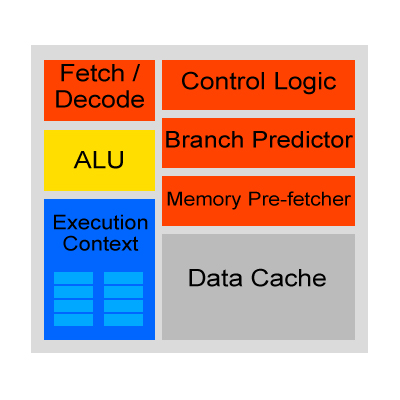
\includegraphics[width=.2\textwidth]{CPU-design.jpg} 
		\captionof{figure}{} 
\end{center}

\begin{center}
	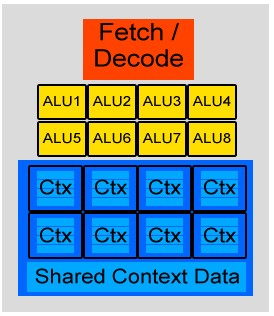
\includegraphics[width=.2\textwidth]{GPU-Design.jpg}
	\captionof{figure}{}
\end{center}

Recently, CPU designers have begun building chips with multiple cores.  This gives the CPU the ability to run SISD and MISD operations well, however there are still performance issues with SIMD and MIMD.  GPU design has been taking advantage of multiple cores per chip for years, and since the archtecture takes up less room than a traditional CPU core, a GPU is capable of fitting many cores on the chip.  This gives the GPU the ability to run SIMD and MIMD operations well.  However, due to the multiple contexts per core, and how the data elements are assigned to these cores, the GPU is not well designed to handle SISD or MISD operations well.

\begin{center}
		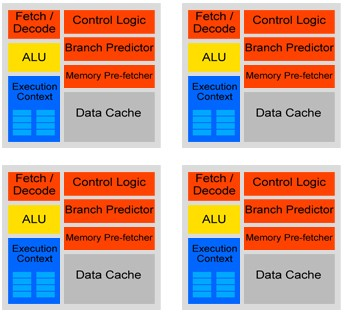
\includegraphics[width=.2\textwidth]{Multicore-CPU-design.jpg} 
		\captionof{figure}{} 
\end{center}

\begin{center}
	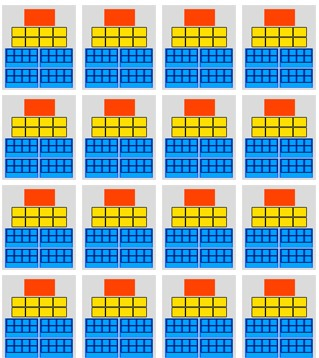
\includegraphics[width=.2\textwidth]{GPU-Design---multiple-cores.jpg}
	\captionof{figure}{}
\end{center}

GPU cores have the ability to modify their context storage areas to vary the number of context elements it holds (by modifying the size of the context elements), which affects the number of context groups for the core to alternate between during computation.  These alternating context groups is how the GPU tries to hide data stalls.  When a group encounters a branch, since there is no forwarding logic, the group must wait for the data.  While this is happening, the core switches to the next group and performs the same instructions that it just executed on the previous group.  By alternating these groups in this manner, called interleaving, the GPU can hide the vast majority of data stalls or branch calculation waits.

\begin{center}
	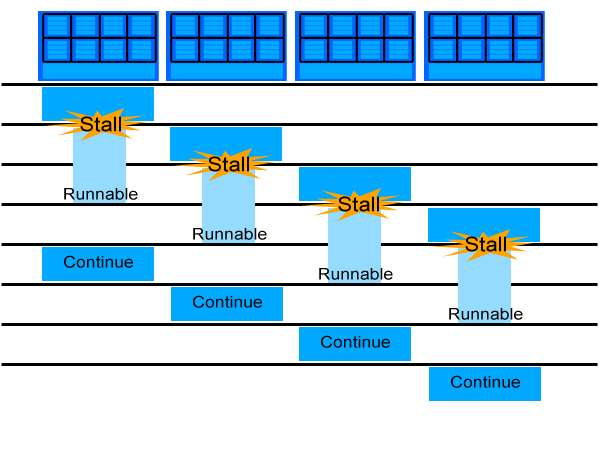
\includegraphics[width=.45\textwidth]{GPU-context-interleaving.jpg}
	\captionof{figure}{}
\end{center}

However, what if the stall time exceeds the amount of time it would take this particular GPU core to alternate amongst all if its context groups?  In this case, there is nothing that can be done to avoid the stall, and the core must wait.  But what if this could be avoided?  Our proposal will endeavor to solve this problem.
\begin{center}
	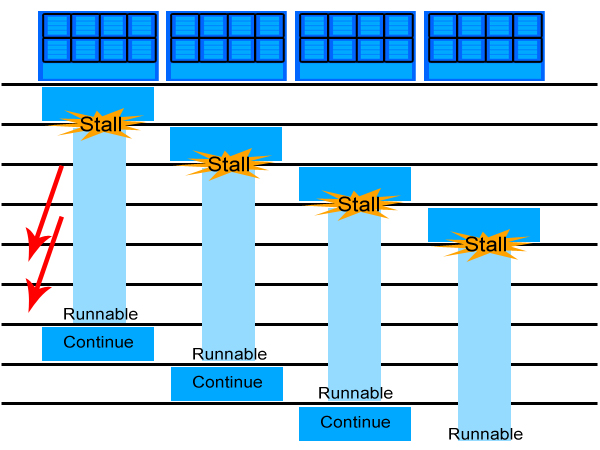
\includegraphics[width=.45\textwidth]{GPU-context-interleaving-2.jpg}
	\captionof{figure}{}
\end{center}

The collection of all context belonging to one GPU core is called a 'warp', and the number of contexts in a warp is  its 'warp factor'.  All contexts within a warp will be subjected to the same instruction stream.  As mentioned before, these contexts will be processed context group by context group.  Due to the nature of how data is assigned to these context elements, there is a great deal of spatial locality amongst the contexts in a warp.  Our proposal believes that there is a way to use the information discovered by the first context group being processed by an instruction stream to assist later context groups in their knowledge of stalls.

On a CPU, each core only has one execution context and one branch prediction table.  This shows that each context handles its own branches and receives no external assistance from other threads.  No external assistance can be offered becuase there is no way to guarantee what the other threads are working on and if it could be useful to the current thread.  In contrast, a GPU core has multiple contexts per core that are all performing the same operations.  Is it possible to use this information to assist other contexts in their branch stalls?

We propose to implement 3 GPU Branch Predictors with the following features:
\begin{itemize}
	\item One predictor is shared amongst the contexts within a GPU core
	\item One predictor is shared only amongst its context group (1 per group)
	\item One predictor is shared only amongst its context (1 per context)
\end{itemize}

\begin{center}
	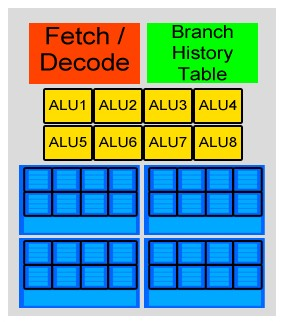
\includegraphics[width=.2\textwidth]{Our-GPU---per-core-predictor.jpg}
	\captionof{figure}{One shared BHT for the entire core.}
\end{center}

\begin{center}
	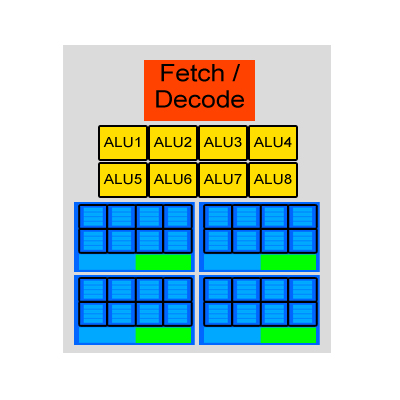
\includegraphics[width=.2\textwidth]{Our-GPU---per-context-group-predictor.jpg}
	\captionof{figure}{One shared BHT for each context group.}
\end{center}

\begin{center}
	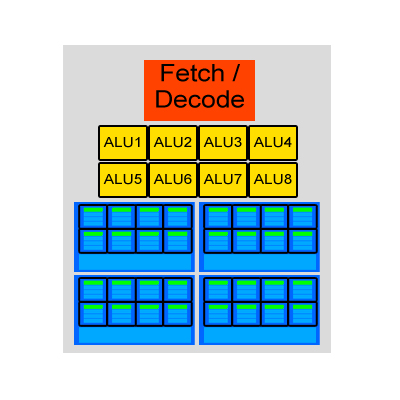
\includegraphics[width=.2\textwidth]{Our-GPU---per-element-predictor.jpg}
	\captionof{figure}{One BHT for each individual context. This implementation most closely resembles how a general CPU would handle branch prediction.}
\end{center}

In addition, the size of the branch history table will be exactly the size of the maximum instruction stream length, which is 16,384 instructions.  We chose this size so that there would be absolutely no predictor collisions, and each instruction location will have its own dedicated predictor.  The predictors we will be using are Smith 2-bit predictors.

\begin{center}
	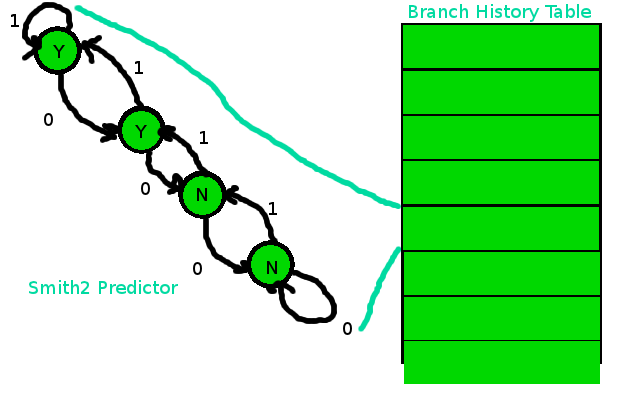
\includegraphics[width=.45\textwidth]{bht.png}
	\captionof{figure}{Smith 2-bit predictor.}
\end{center}

We will compare prediction accuracies across these three implementations.  Our goal is that after the initial training of the predictors, the GPU cores will process their contexts groups as shown in the figure below:

\begin{center}
	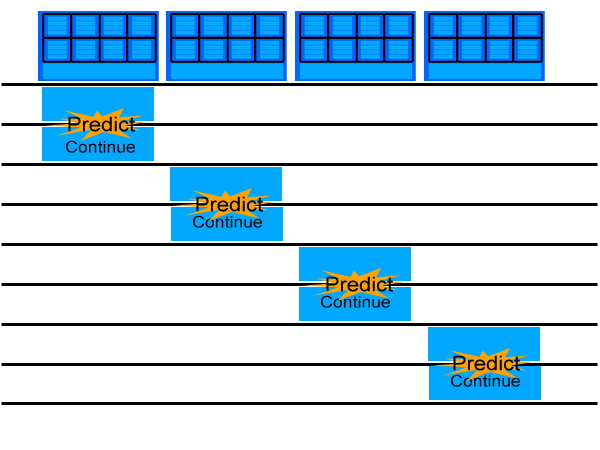
\includegraphics[width=.45\textwidth]{GPU-predict-context.jpg}
	\captionof{figure}{Context interleaving is not necessary, as the groups are properly predicting where to branch and continue operation.}
\end{center}

\section{Simulation Methodology}

In order to properly model our proposal, we must have an appropriate simulator modeling SIMD/SIMT architecture.  The SimpleScalar simulator was not sufficient, as it simulates CPU behaviors (including all of the behaviors that are removed from GPUs).  Due to our truncated timetable, we couldn't properly modify SimpleScalar, so we needed to find a GPU-specific simulator.  We found GPGPU-Sim, which is a rewrite based on the SimpleScalar simulator.  This simulator simulates an NVIDIA Quadro 5800 graphics card, with the following statistics:

\begin{itemize}
	\item 16k register file
	\item 4 GB RAM
	\item 32 GPU cores
	\item 1024 contexts
\end{itemize}

This simulator creates libcuda.so and libOpenCL.so files on the fly to intercept GPU commands from CPU program during execution.  This method of execution requires NVIDIA hardware to build benchmarks because the driver does the compilations.

\begin{center}
	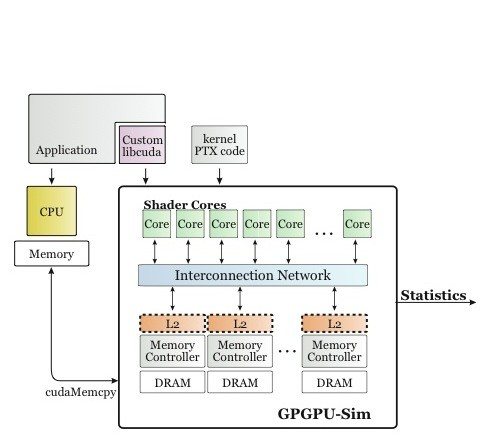
\includegraphics[width=.45\textwidth]{uarch1.jpg}
	\captionof{figure}{GPGPU-Sim architecture.}
\end{center}

\begin{center}
	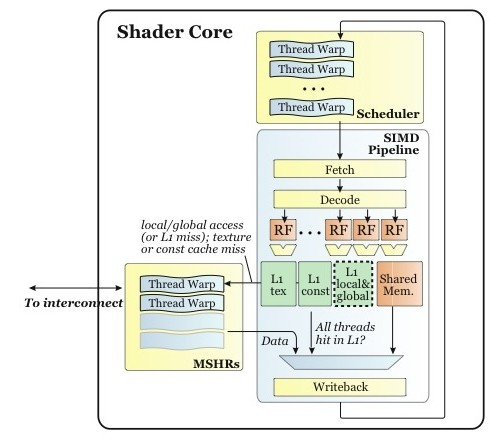
\includegraphics[width=.45\textwidth]{uarch2.jpg}
	\captionof{figure}{GPGPU-Sim Shader core.}
\end{center}

Since we are simulating GPU hardware, it is important to run our simulator on GPU-specific benchmarks as gcc, gzip, and other common benchmarks are designed to benchmark CPU hardware changes.  We settled on using a subset of ISPASS09 CUDA benchmarks.  We used a subset of these benchmarks because some of them were failing right out of the box.  One benchmark ran continuously for 4 days before we decided to kill it and not use it.  Other benchmarks said the CPU component was failing to meet its dependencies or that the CUDA architecture was unsupported (double precision vs. single precision computations).  Yet another benchmark was written so well that it had no branching instructions during execution at all.

After deciding which benchmarks weren't going to show us anything useful (or run in a nominal amount of time for our deadlines), we settled on a suite of four benchmarks:

\begin{itemize}
	\item \emph{NQU} - Solving the NQUEENS problem
	\item \emph{NN} - Classification of images with a neural net
	\item \emph{RAY} - Raytracing a scene
	\item \emph{BFS} - Breadth-First Search of a graph
\end{itemize}

\section{Simulation Results}

After running our implementations through our benchmark suite, we noticed a few interesting things.  First, we saw significant improvements in prediction accuracy in the per group and per core predictors when compared to the per context predictor.  The per context predictors on \emph{BFS} scored nearly an 18\% miss rate.  However, both the per group and per core predictors scored amazing 0.9\% and 0.8\% miss rates, respectively.  While not as huge of an improvement as with the \emph{BFS}, the per group and per core predictors posted very respectable improvements over the per context predictor while operating on \emph{NN} and \emph{RAY}.

Second, we noticed that the per group and per core predictors performed worse than the per context predictor while operating on the \emph{NQU} benchmark.  It is possible that this occurred due to the nature of the \emph{NQU} problem, which does not exhibit the same kind of spatial locality as would be required to take advantage of either the per group or per core predictors.

\begin{center}
	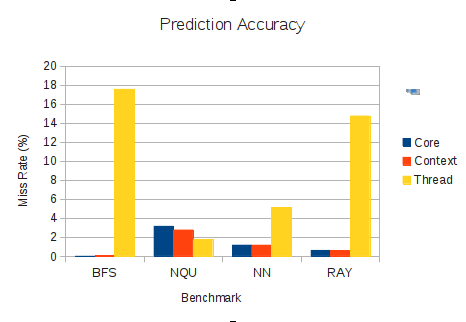
\includegraphics[width=.45\textwidth]{data.png}
	\captionof{figure}{}
\end{center}

\section{Conclusions}

\section{References}

\bibliographystyle{IEEEtran}
\bibliography{IEEEabrv,gpu_predict_paper}


% An example of a floating figure using the graphicx package.
% Note that \label must occur AFTER (or within) \caption.
% For figures, \caption should occur after the \includegraphics.
% Note that IEEEtran v1.7 and later has special internal code that
% is designed to preserve the operation of \label within \caption
% even when the captionsoff option is in effect. However, because
% of issues like this, it may be the safest practice to put all your
% \label just after \caption rather than within \caption{}.
%
% Reminder: the "draftcls" or "draftclsnofoot", not "draft", class
% option should be used if it is desired that the figures are to be
% displayed while in draft mode.
%
%\begin{figure}[!t]
%\centering
%\includegraphics[width=2.5in]{myfigure}
% where an .eps filename suffix will be assumed under latex, 
% and a .pdf suffix will be assumed for pdflatex; or what has been declared
% via \DeclareGraphicsExtensions.
%\caption{Simulation Results}
%\label{fig_sim}
%\end{figure}

% Note that IEEE typically puts floats only at the top, even when this
% results in a large percentage of a column being occupied by floats.


% An example of a double column floating figure using two subfigures.
% (The subfig.sty package must be loaded for this to work.)
% The subfigure \label commands are set within each subfloat command, the
% \label for the overall figure must come after \caption.
% \hfil must be used as a separator to get equal spacing.
% The subfigure.sty package works much the same way, except \subfigure is
% used instead of \subfloat.
%
%\begin{figure*}[!t]
%\centerline{\subfloat[Case I]\includegraphics[width=2.5in]{subfigcase1}%
%\label{fig_first_case}}
%\hfil
%\subfloat[Case II]{\includegraphics[width=2.5in]{subfigcase2}%
%\label{fig_second_case}}}
%\caption{Simulation results}
%\label{fig_sim}
%\end{figure*}
%
% Note that often IEEE papers with subfigures do not employ subfigure
% captions (using the optional argument to \subfloat), but instead will
% reference/describe all of them (a), (b), etc., within the main caption.


% An example of a floating table. Note that, for IEEE style tables, the 
% \caption command should come BEFORE the table. Table text will default to
% \footnotesize as IEEE normally uses this smaller font for tables.
% The \label must come after \caption as always.
%
%\begin{table}[!t]
%% increase table row spacing, adjust to taste
%\renewcommand{\arraystretch}{1.3}
% if using array.sty, it might be a good idea to tweak the value of
% \extrarowheight as needed to properly center the text within the cells
%\caption{An Example of a Table}
%\label{table_example}
%\centering
%% Some packages, such as MDW tools, offer better commands for making tables
%% than the plain LaTeX2e tabular which is used here.
%\begin{tabular}{|c||c|}
%\hline
%One & Two\\
%\hline
%Three & Four\\
%\hline
%\end{tabular}
%\end{table}


% Note that IEEE does not put floats in the very first column - or typically
% anywhere on the first page for that matter. Also, in-text middle ("here")
% positioning is not used. Most IEEE journals/conferences use top floats
% exclusively. Note that, LaTeX2e, unlike IEEE journals/conferences, places
% footnotes above bottom floats. This can be corrected via the \fnbelowfloat
% command of the stfloats package.


% trigger a \newpage just before the given reference
% number - used to balance the columns on the last page
% adjust value as needed - may need to be readjusted if
% the document is modified later
%\IEEEtriggeratref{8}
% The "triggered" command can be changed if desired:
%\IEEEtriggercmd{\enlargethispage{-5in}}

% references section

% can use a bibliography generated by BibTeX as a .bbl file
% BibTeX documentation can be easily obtained at:
% http://www.ctan.org/tex-archive/biblio/bibtex/contrib/doc/
% The IEEEtran BibTeX style support page is at:
% http://www.michaelshell.org/tex/ieeetran/bibtex/
%\bibliographystyle{IEEEtran}
% argument is your BibTeX string definitions and bibliography database(s)
%\bibliography{IEEEabrv,midterm.bib}
%
% <OR> manually copy in the resultant .bbl file
% set second argument of \begin to the number of references
% (used to reserve space for the reference number labels box)

%\begin{thebibliography}{1}

%\bibitem{IEEEhowto:kopka}
%H.~Kopka and P.~W. Daly, \emph{A Guide to \LaTeX}, 3rd~ed.\hskip 1em plus
%  0.5em minus 0.4em\relax Harlow, England: Addison-Wesley, 1999.

%\end{thebibliography}

%\bibliographystyle{ieeetr}
%\bibliography{midterm}

%\appendix
%\section{Project Progress}
%\subsection{Challenges Encountered}
%\subsection{Completed Tasks}
%\subsection{Remaining Tasks}


% that's all folks
%\bibliographystyle{ieeetr}
%\bibliography{midterm}




%\appendix
%\section{Project Progress}
%\subsection{Challenges Encountered}
%\subsection{Completed Tasks}
%\subsection{Remaining Tasks}

\end{document}


